\documentclass[a4,12pt]{book}
\usepackage[portuguese]{babel}
\usepackage[utf8]{inputenc}
\usepackage[portugues]{mystyle}
\usepackage{multirow}
\usepackage{multicol}
\usepackage{rotating}
\usepackage{amsmath}
\usepackage{tikz}
\usepackage{tikz-qtree}
\usepackage{clrscode}
\usepackage[hidelinks]{hyperref}
\usetikzlibrary{automata, positioning, decorations.pathmorphing}
\usepackage{biblatex}
\addbibresource[label=bib]{ref.bib}
\usepackage{listings}


\emergencystretch=2em

\DeclareFontFamily{U}{matha}{\hyphenchar\font45}
\DeclareFontShape{U}{matha}{m}{n}{
      <5> <6> <7> <8> <9> <10> gen * matha
      <10.95> matha10 <12> <14.4> <17.28> <20.74> <24.88> matha12
      }{}
\DeclareSymbolFont{matha}{U}{matha}{m}{n}
\DeclareFontSubstitution{U}{matha}{m}{n}
\DeclareMathSymbol{\abxcup}{\mathbin}{matha}{'131}

\newcounter{mycounter}
\setcounter{mycounter}{0}
\newenvironment{exercicio}{\refstepcounter{mycounter}
    {\bf Exercício~\themycounter: }
      \rmfamily}{\medskip}

\begin{document}

%\bibliographystyle{alpha}

\author{Márcio Moretto Ribeiro}

\title{Introdução à Análise de Algoritmos}

\maketitle
\tableofcontents

\chapter*{Apresentação}

Esta apostila são notas de aula do curso ministrado por mim no segundo semestre de 2021 para as duas turmas noturnas de Sistemas de Informação ministrado à distância por conta da pandemia de COVID19.
Seu conteúdo está baseado nos livros que servem de bibliografia para o curso:

\nocite{sedgewick01,sedgewick11,cormen12}


\printbibliography[heading=none,keyword={bibliografia}]

%\begin{thebibliography}
%\bibitem{sedgewick11}
%\bibitem{sedgewick01}
%\bibitem{cormen12}
%\end{thebibliography}

  Além dos livros serviu de material para elaboração dessas notas outros textos citados ao longo do curso bem como as gravações dos cursos do professor Robert Sedgeweick para o Coursera e do professor Ronald Rivest para o MIT.

  
  A última versão desta apostila está disponível em um repositório no github (https://github.com/marciomr/apostila-iaa.git).
  Agradeço de antemão eventuais sugestões de correção que forem submetidas pela plataforma.

  Alguns dos direitos sobre o conteúdo desta apostila estão protegidos pela licensa Creative Commons Attribution-NonCommercial-ShareAlike 4.0 International (CC BY-NC-SA 4.0).
Ou seja, você  é livre para distribuir cópias e adaptar este trabalho desde que mantenha a mesma licença, dê o devido crédito ao autor e não faça uso comercial.

\begin{center}
  
\includegraphics[width=.3\textwidth]{imagens/cc.png}
\end{center}

\chapter{Introdução}

\section{Apresentação}

Esta apostila são notas de aula do curso ministrado por mim no segundo semestre de 2021 para as duas turmas noturnas de Sistemas de Informação ministrado à distância por conta da pandemia de COVID19.
Seu conteúdo está baseado nos livros que servem de bibliografia para o curso:

\nocite{sedgewick01,sedgewick11,cormen12}


\printbibliography[heading=none,keyword={bibliografia}]

%\begin{thebibliography}
%\bibitem{sedgewick11}
%\bibitem{sedgewick01}
%\bibitem{cormen12}
%\end{thebibliography}

  Além dos livros serviu de material para elaboração dessas notas outros textos citados ao longo do curso bem como as gravações dos cursos do professor Robert Sedgeweick para o Coursera e do professor Ronald Rivest para o MIT.

  
  A última versão desta apostila está disponível em um repositório no github (https://github.com/marciomr/apostila-iaa.git).
  Agradeço de antemão eventuais sugestões de correção que forem submetidas pela plataforma.

  Alguns dos direitos sobre o conteúdo desta apostila estão protegidos pela licensa Creative Commons Attribution-NonCommercial-ShareAlike 4.0 International (CC BY-NC-SA 4.0).
Ou seja, você  é livre para distribuir cópias e adaptar este trabalho desde que mantenha a mesma licença, dê o devido crédito ao autor e não faça uso comercial.

\begin{center}
  
\includegraphics[width=.3\textwidth]{imagens/cc.png}
\end{center}

\section{Algoritmos}

Um {\em problema computacional} é a especificação de uma relação desejada entre um certo {\em valor de entrada} escolhido em um conjunto de valores válidos e o {\em valor de saída} esperado.

\begin{example}
  {\bf Problema da busca}\\

  {\bf Entrada:} Uma sequência de $n \in \mathbb{N}$ valores $\langle a_1, \dots, a_n \rangle$ em que $a_i \in \mathbb{Z}$ para $1 \leq i \leq n$ e $b \in \mathbb{Z}$.\\

  {\bf Saída:} $i \in \mathbb{N}$ tal que $a_i = b$ se existir ou $\bot$ caso contrário.
\end{example}

\begin{example}
  {\bf Problema da 3-soma}\\

  {\bf Entrada:} Três sequência de $n \in \mathbb{N}$ valores cada $\langle a_1, \dots, a_n \rangle$,  $\langle b_1, \dots, b_n \rangle$ e $\langle c_1, \dots, c_n \rangle$ em que $a_i, b_i, c_i \in \mathbb{Z}$ para $1 \leq i \leq n$.\\

  {\bf Saída:} O número $m \in \mathbb{N}$ de $i, j, k \in \mathbb{N}$ tal que $a_i + b_j + c_j = 0$.
\end{example}

\begin{example}
  {\bf Problema da ordenação}\\

  {\bf Entrada:} Uma sequência de $n \in \mathbb{N}$ valores $\langle a_1, \dots, a_n \rangle$ em que $a_i \in \mathbb{Z}$ para $1 \leq i \leq n$.\\

  {\bf Saída:} Uma permutação da sequência de entrada $\langle a'_1, \dots, a'_n \rangle$ tal que $a_i \leq a_j$ para todo $i \leq j$.
\end{example}

Uma {\em instância do problema} consiste de uma entrada válida para a qual se pretende produzir uma saída esperada.
Por exemplo, a sequência $\langle 3, 42, 17, 2, -1 \rangle$ é uma instância do problema da ordenação cuja saída esperada é $\langle -1, 2, 3, 17, 42 \rangle$.

A disciplina de Introdução à Teoria da Computação (ITC) tem como objeto de estudo problemas computacionais, como eles se classificam entre os que tem solução ou não e entre os que tem solução eficiente ou não.
A solução de um problema computacional é um algoritmo.

Os objetos de estudo desta disciplina são os algoritmos.
Mas afinal, o que são algoritmos?

Um {\em algoritmo} parte de uma entrada escolhida em um conjunto potencialmente infinito de possibilidades ({\em princípio da massividade}) para produzir um valor de saída.
O algoritmo processa a entrada por meio de uma sequência de passos ({\em princípio da discretude}) que produzem valores intermediários.
Cada passo  segue uma instrução simples ({\em princípio da elementaridade}) que só depende dos valores anteriores, não admitindo ambiguidades ({\em princípio da exatidão}) \cite{malcev70}.

Um {\em prorgrama} é a realização de um algoritmo em certa {\em linguagem de programação}.
Assim, um algoritmo é, de um lado, a solução de um problema de computação e, de outro, uma abstração de um conjunto de programas, ele é a idéia por trás do programa.

Um algoritmo é {\em correto} se para toda instância do problema ele produz a saída esperada depois de uma sequência finita de passos.
Nesse caso dizemos que o algoritmo {\em resolve} o problema.

Há uma controversa se devemos ou não considerar uma sequência infinita de instruções como um algoritmo.
Essa questão, complicada, está no coração do nascimento da ciência da computação e será tratada em ITC.
Neste curso focaremos nos algoritmos corretos e, assim, escaparemos da questão.

Para enfatizar o fato de que um algoritmo é uma abstração de um programa, eles serão apresentados neste curso em uma linguagem informal conhecida como {\em pseudo-código}.

\begin{example}
  Considere a seguinte solução para o problema da busca.

\begin{codebox}
\Procname{$\proc{BuscaSimples}(A, b)$}
\li \Comment Recebe $\langle a_1, \dots, a_n \rangle \in \mathbb{Z}^n$ e $b \in \mathbb{Z}$
\li \Comment Devolve $i$ tal que $a_i = b$ se existir e $\bot$ caso contrário
\li \For $i \gets 1$ até $n$
\li \Do \If $a_i = b$
\li     \Then \Return $i$
        \End
    \End
\li \Return $\bot$
\End
\end{codebox}
  
\end{example}

Esta disciplina estuda algoritmos.
Como podemos garantir que certo algoritmo resolve um problema, ou seja, que ele é correto?
Como podemos comparar duas soluções distintas para um mesmo problema?
Ou seja, se conhecemos dois um mais algoritmos corretos para um mesmo problema, como avaliamos qual é melhor?

Avaliaremos os algoritmos corretos a partir da quantidade de recursos que ele consome.
Estudaremos particularmente dois recursos: espaço de memória e, principalmente, o tempo de execução.

Nos capítulos seguintes veremos uma série de algoritmos para resolver alguns problemas centrais da computação como o problema da busca e da ordenação.
Avaliaremos os algoritmos apresentado quanto sua corretude e sua eficiência em consumo de tempo e espaço de memória.

No Capítulo X apresentaremos o estudo dos algoritmos a partir do método empírico.
Relembraremos o método e veremos um exemplo comparando o tempo de execução de duas soluções para o problema da busca em sequências ordenadas.
Então exploraremos técnicas para arrsicar modelos matemáticos adequados para avaliar o consumo de tempo dos algoritmos.
E finalmente veremos ferramentas matemáticas uteis para comparar funções quanto ao seu crescimento, a chamada notação assintótica.
No Capitulo X estudaremos algoritmos de ordenação como estudo de caso da teoria apresentada anteriormente.
Veremos uma série de algoritmos que resolvem o mesmo problema e utilizaremos as técnicas apresentadas para construir e testar modelos do consumo de tempo deles.
Estudaremos também um limite teórico da eficiência do problema da ordenação e veremos dois algoritmos que superam esse limite utilizando mais informações do que as assumidas no enunciado do teorema.
Concluiremos a apostila no Capítulo X apresentando algoritmos e técnicas um pouco mais avançãdos como programação dinâmica e análise amortizada.


\chapter{Método Empírico}

Esquematicamente, o método empírico pode ser descrito por cinco fases:
\begin{enumerate}
\item {\em Observação:} medições sobre algum aspecto do mundo
\item {\em Hipótese:} concepção de um modelo consistente com as observações
\item {\em Predição:} eventos são previstos de acordo com o modelo
\item {\em Verificação:} as predições são testadas fazendo-se novas observações
\item {\em Validação:} o processo se repete ajustando o modelo até que ele concorde com as observações
\end{enumerate}

Dois pontos centrais sobre o método empírico é que as verificações devem ser {\em reprodutíveis} e as hipóteses {\em falseáveis}.
Uma hipóstese que não pode ser falseada por observações (empíricamente) não é científica e a o processo de verificação deve poder ser feito por outros cientístas independentes.

O aspecto do mundo que pretendemos investigar nesta disciplina é o tmepo de processamento de um algoritmo.
Lembre-se, porém, que um algoritmo é uma ideia que precede o advento dos computadores.
O algoritmo de Euclídes, por exemplo, data de 300 a.C., ou seja, séculos antes dos primeiros computadores começarem a ser construídos nos anos 40.
Embora o algoritmo seja um conceito matemático, uma série de pesquisadores tiveram a ideia de investigá-los de maneira empírica no final dos anos 60.
A série de livros The Art of Programing, de Donald Knuth, é um marco dessa abordagem dos estudos de algoritmos \cite{knuth97}.

Em nosso recorte, observaremos o tempo de processamento da execução de um programa para diferentes entradas.
Considere, por exemplo, o algoritmo para o problema da Busca apresentado no capítulo anterior:

\begin{codebox}
\Procname{$\proc{BuscaSequencial}(A, b)$}
\li \For $i \gets 1$ até $n$
\li \Do \If $a_i = b$
\li     \Then \Return $i$
        \End
    \End
\li \Return $\bot$
\End
\end{codebox}

Vamos implementar esse algoritmo na linguagem C de maneira direita:

\begin{lstlisting}[language=C]
  // devolve a posicao de n no arranjo ou -1 se nao encontrar
  int buscasequencial(int* array, int n, int size){
    int i;
    for(i = 0; i < size; i++)
      if(array[i] == n)
        return i;
    return -1;
  }      
\end{lstlisting}

Realizamos observações usando uma máquina específica (um notebook Dell com processador intel core i7 de $8^a$ geração de 1,9GHz) em um sistema operacional específico (Linux 5.11).
Medimos o tempo total de 300 buscas mal sucedidas em arranjos de tamanhos diferentes com valores inteiros positivos calculados aleatoriamente\footnote{Mais precisamente os valores seguem uma sequência pseudo-aleatória partindo de uma semente incial.}.
Os programas que calcula o tempo da busca e que gera as entradas estão disponíveis em \url{https://github.com/marciomr/IAA}.
Variamos o tamanho do arranjo entre um milhão e dez milhões.
Obtivemos o seguinte resultado para dez observações:

\begin{table}
  \label{tab:observacao}
  \begin{tabular}{|c|c|}
    \hline
    tamanho do arranjo em milhões & tempo de 300 buscas em segundos \\
    \hline 
    1                             & 0,99                            \\
    2                             & 2,08                            \\
    3                             & 3,12                            \\
    4                             & 3,99                            \\
    5                             & 5,05                            \\
    6                             & 5,94                            \\
    7                             & 7,03                            \\
    8                             & 7,92                            \\
    9                             & 8,93                            \\
    10                            & 9,85                            \\
    \hline
  \end{tabular}
\end{table}

As observações sugerem que para cada um milhão de valores no arranjo, o tempo de processamento aumenta mais ou menos um segundo.
Essa poderia ser nossa hipótese, mas podemos fazer algo um pouco mais sofisticado.
Vamos plotar os valores da tabela em um gráfico (Figura \ref{fig:observacao}).

\begin{figure}[htp]
  \label{fig:observacao}
  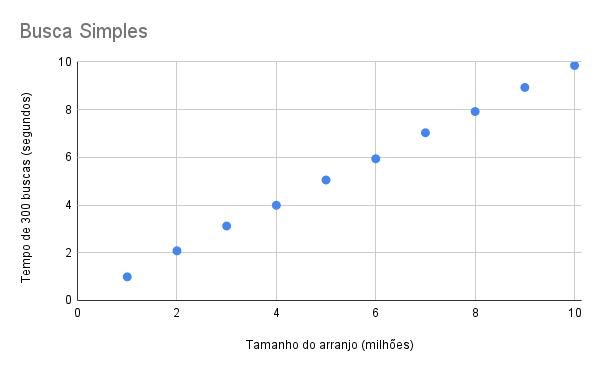
\includegraphics[width=0.9\textwidth]{imagens/grafico1.png}
  \caption{Tempo de processamento da busca simples.}
\end{figure}

Como os pontos estão mais ou menos alinhados e como é razoável supor que um arranjo sem nenhum elemento retornaria instantaneamente o resultado, faremos a hipótese de que o tempo de processamento segue uma função linear partindo do zero.
Ou seja, a seguinte função descreve o tempo de processamento da nossa implementação em nosso ambiente:

\begin{displaymath}
t(x) = a.x
\end{displaymath}

Podemos então usar uma regressão linear para estimar o valor de $a$ que minimize a distância desse reta para cada um dos pontos.
Obtemos então o valor $a = 0,997$.
Na Figura \ref{fig:hipotese} plotamos a função $t(x) = 0,997x$ no gráfico anterior.

\begin{figure}[htp]
  \label{fig:hipotese}
  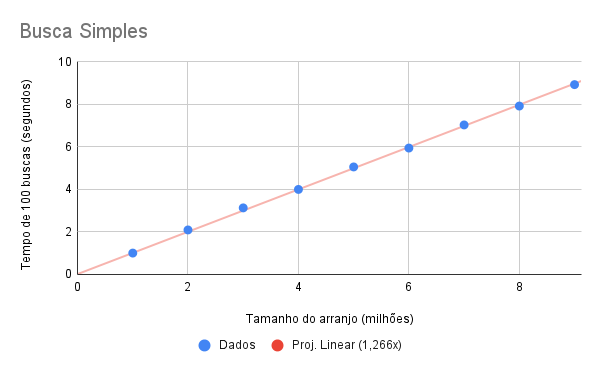
\includegraphics[width=0.9\textwidth]{imagens/grafico2.png}
  \caption{Gráfico ilustrando a hipótese de que o tempo de processamento da busca simples segue a função $t(x) = 0,997x$.}
\end{figure}

Podemos agora testar nossa hipótese de que o tempo de processamento da nossa implementação da busca sequencial para outros valores ainda não observados.
A segunda coluna da Tabela \ref{tab:verificacao} mostra os valores previstos pela hipótese para o tempo de processamento para entradas de tamanho 11 a 15 milhões.
Finalmente, podemos testar a hipótese.
Na última coluna da mesma tabela indicamos os valores observados para essas entradas:

\begin{table}
  \label{tab:verificacao}
  \begin{tabular}{|c|c|c|}
    \hline
    tamanho do arranjo em milhões & tempo previsto & tempo observado \\
    \hline 
    11                             & 10,97         & 10,87           \\
    12                             & 11,97         & 11,81           \\
    13                             & 12,97         & 12,78           \\
    14                             & 13,96         & 14,00           \\
    15                             & 14,96         & 14,74           \\
    \hline
  \end{tabular}
  \caption{Tempo de processamento previsto e observado para tamanhos maiores de arranjos.}
\end{table}

Os valores observados são notavelmente próximos aos previstos.
Ou seja, nossa hipótese foi verificada.
Poderíamos neste momento utilizar um teste estatístico para verificar nossa hipótese, mas isso foge do escopo desta disciplina.
Por hora diremos apenas que os dados parecem verificar a hipótese.



\printbibliography

%\bibliography{ref}
\end{document}
